\documentclass[main]{subfiles}

\begin{document}


\chapter{Pruebas del controlador}
El controlador diseñado se comporta adecuadamente en lo que respecta a las simulaciones, sin embargo debido a que la caracterizaci\'on del sistema puede contener errores se procede a realizar algunas pruebas sobre los subsistemas que componen al sistema global como paso intermedio antes de realizar una prueba de vuelo real. Estas pruebas son de utilidad para verificar el correcto funcionamiento del controlador diseñado y/o para realizar los ajustes que sean necesarios en el mismo.

\section{Control de subsistemas Roll y Pitch}

Para lograr que el cuadric\'optero se mantenga horizontal, es fundamental que el control sobre los \'angulos de Pitch y de Roll se comporten de acuerdo a lo esperado. A modo de ejemplo, es imposible lograr el equilibrio mec\'anico si dichos \'angulos difieren de cero. Por dicha raz\'on, previo a realizar pruebas sobre el sistema completo es necesario asegurarnos que los subsistemas de  Roll y Pitch funcionan correctamente. De acuerdo al modelo f\'isico del sistema desarrollado en \ref{chap:modelo} ni el Roll ni el Pitch son subsistemas independientes entre s\'i, adem\'as ambos dependen de la velocidad angular seg\'un $\vec{k}_q$. Sin embargo, dichos \'angulos toman valores cercanos a cero en las trayectorias de inter\'es, caso en el cual se puede realizar la aproximaci\'on de que ambos sistemas son independientes.\\

A continuación se explicará solamente el funcionamiento para el ángulo de Roll, ya que para Pitch el procedimiento es completamente análogo.\\

\begin{wrapfigure}{r}{0.55\textwidth}
	\vspace{-20pt}
	\centering
	\includegraphics[width=0.4\textwidth]{./pics_test_control/dispositivo_psi.pdf}
	\caption{Dispositivo de prueba de Roll}
	\label{fig:psidisp}
	\vspace{-20pt}
\end{wrapfigure}

A partir de esta consideraci\'on se procede a fijar al cuadric\'optero sobre dos gu\'ias como se muestra en la figura \ref{fig:psidisp}, de forma de eliminar todos los grados de libertad del sistema excepto el \'angulo de Roll ($\psi$) y la velocidad angular correspondiente al eje de rotaci\'on de este ángulo. Se realizan dos pruebas: la primera consiste en que el sistema alcance la posici\'on de equilibrio ($\psi = 0$), la segunda consiste en alejar al sistema del equilibrio y lograr que vuelva al punto de equilibrio.\\

El controlador posee dos términos proporcionales: uno para el \'angulo $\psi$ y el otro para la velocidad angular $\omega_{qx}$. Además se considera un t\'ermino integral asociado a la integral de $\psi$. El modelo de este subsistema es el siguiente:
\begin{equation}
\left(\begin{array}{c}
\dot{\psi}\\
\dot{\omega}_{qx}\\
\dot{\psi_I}
\end{array}\right) = \left(\begin{array}{ccc}
0 & 1 & 0\\
-\frac{MgL^\prime}{I_{xx}} & 0 & 0\\
1 & 0 &0
\end{array}\right) 
\left(\begin{array}{c}
{\psi}\\
{\omega}_{qx}\\
{\psi_I}
\end{array}\right)
+ b\left(\begin{array}{cc}
0 & 0\\
1 & -1\\
0 & 0\\
\end{array}\right) \left(\begin{array}{c}
\omega_2 \\
\omega_4
\end{array}\right)
\end{equation}

donde $b$ y $\frac{MgL^\prime}{I_{xx}}$ se calculan a partir de las caracterizaciones realizadas anteriormente. La matriz Q difiere de la utilizada en las simulaciones ya que el error sistem\'atico implicaba tiempos de correcci\'on del \'angulo mayores a lo aceptable. Se utilizan las matrices $Q$ y $R$:
\begin{equation}
\label{eq:Q_R_roll}
Q = \left(\begin{array}{ccc}
1000 & 0 & 0\\
0 & 1 & 0\\
0 & 0 & 100 
\end{array} \right) \quad R =\left(\begin{array}{cc}
0.1 & 0 \\
0 & 0.1
\end{array}\right)
\end{equation}
la matriz de realimentaci\'on obtenida es la mostrada en la ecuación \ref{K_roll}
\begin{equation}
\label{K_roll}
K = \left( \begin{array}{ccc}
44.43 & 10.78 &21.36\\
-44.430 & -10.78 &-21.36
\end{array}\right)
\end{equation}

\begin{wrapfigure}{r}{0.6\textwidth}
	\vspace{-10pt}
	\centering
	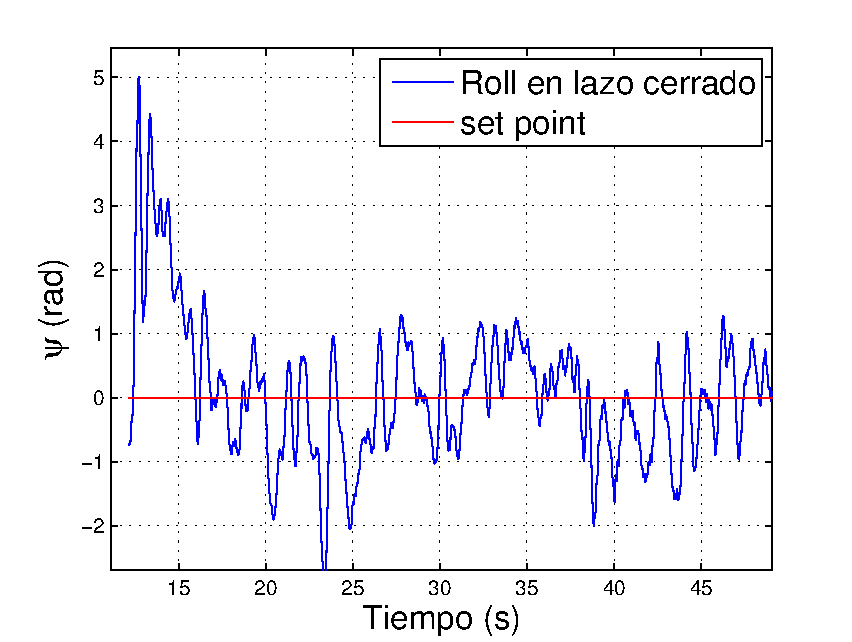
\includegraphics[width=0.52\textwidth]{./pics_test_control/psi.pdf}
	\caption{\'Angulo de Roll en lazo cerrado}
	\label{fig:psi}
\end{wrapfigure}
\vspace{10pt}
En la figura \ref{fig:psi} se observa la respuesta del \'angulo de Roll en lazo cerrado, con el setpoint fijo en $\psi = 0$. Se observa que el m\'odulo del \'angulo es siempre inferior a los $2^\circ$ a excepci\'on del arranque y algún pico aislado. Se puede decir que presenta un error típico de $\pm 1^\circ$. En este sentido se puede afirmar que el control implementado es exitoso, ya que logra el objetivo planteado. Puede observarse adem\'as que una vez que el controlador comienza a actuar se produce un cambio en el \'angulo alcanzando un valor cercano a los $5 ^\circ$. Este error es producido por la diferencia del empuje de los motores frente a una misma orden. El control integral es el encargado de corregir esta diferencia en aproximadamente $2.5$ segundos, tiempo que dependiendo de la aplicación puede ser o no aceptable. Un ángulo de algunos grados durante 2 segundos provocará un desplazamiento que puede llegar a ser inaceptable dependiendo de la aplicación. Como se sabe que es causado por una no idealidad sobre el empuje de los motores ante igual comando, es posible evitar este desplazamiento inicial muy fácilmente con tan solo inicializar al integrador en algún valor apropiado (distinto de cero). De esta forma se logra un despegue más prolijo ya que el ángulo $\psi$ permanecerá todo el tiempo más cerca de cero.\\

Ante este tipo de imperfecciones el control proporcional es el encargado de volver a estabilizar al cuadricóptero, pero lo hará en algún otro punto de equilibrio que no necesariamente es el deseado. Por otro lado es el control integral el encargado de que el cuadricóptero alcance el equilibrio deseado, que será probablemente distinto al equilibrio hallado por el proporcional.\\

\begin{wrapfigure}{r}{0.57\textwidth}
	\centering
	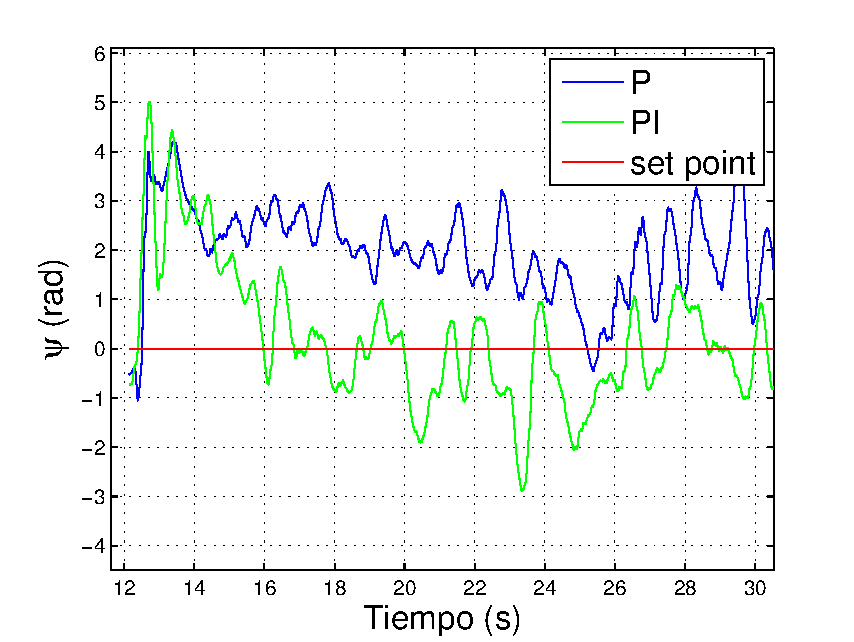
\includegraphics[width=0.48\textwidth]{./pics_test_control/psi_sin_con_int.pdf}
	\caption{\'Angulo de Roll en lazo cerrado}
	\label{fig:psi_sin_con_int}
\end{wrapfigure}

En la figura \ref{fig:psi_sin_con_int} se puede observar la diferencia entre utilizar un controlador puramente proporcional y un controlador proporcional con una correcci\'on integral. El primero no logra corregir el error sistem\'atico debido a la diferencia en el empuje de los motores alcanzando as\'i un punto de equilibrio distinto del \emph{set point}. El controlador con el t\'ermino integral s\'i logra corregir este error y el \'angulo $\psi$ toma valores en el entorno del \emph{set point}.\\


\begin{wrapfigure}{l}{0.52\textwidth}
	\vspace{-10pt}
	\centering
	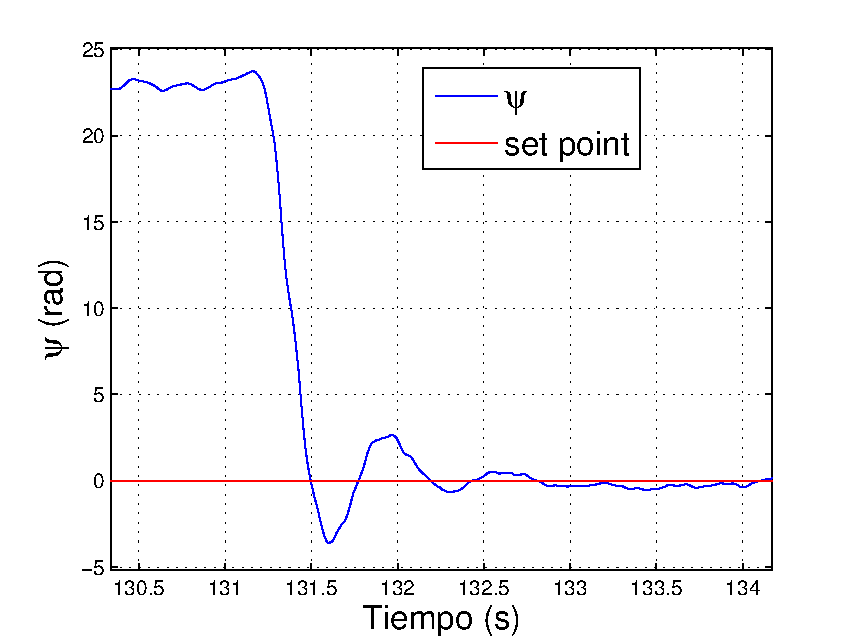
\includegraphics[width=0.48\textwidth]{./pics_test_control/psi_esc.pdf}
	\caption{Respuesta al escal\'on de Roll\\ en lazo cerrado}
	\label{fig:psi_esc}
\end{wrapfigure}

Resulta fundamental entender como es la respuesta del sistema realimentado para apartamientos considerables respecto del equilibrio. Dicha situaci\'on puede producirse por diversas razones, un leve golpe de alg\'un agente externo o una simple turbulencia. En la figura \ref{fig:psi_esc} puede observarse la respuesta al escal\'on del sistema en lazo cerrado	con \'angulo inicial de aproximadamente $23 ^\circ$ y \emph{set point} $0 ^\circ$. La respuesta del sistema es muy buena, ya que se logra el valor de \emph{set point} en aproximadamente un segundo y la misma presenta un sobretiro del orden del $10\%$, obteniendo un resultado sumamente satisfactorio.\\

Con este an\'alisis se concluye que la matriz de realimentaci\'on obtenida es adecuada para controlar el subsistema del \'angulo de Roll.

\section{Control del subsistema del Yaw}

De manera an\'aloga al caso anterior, es importante verificar el buen funcionamiento del control sobre el giro en ``z'', para lo cual se utiliza un dispositivo de prueba que restringe los grados de libertad del cuadric\'optero. En este caso se lo sujeta con una cuerda desde arriba de los cuatro brazos de modo de realizar la fuerza lo m\'as pareja posible, como se muestra en la figura \ref{fig:thetadisp}. El cuadric\'optero queda sujetado colgando horizontal y conserva el libre giro seg\'un ``z'' ($\theta$).
Se setea una velocidad de \emph{hovering} inferior a la necesaria para levantar vuelo, de modo que el cuadric\'optero no se eleve y la cuerda quede siempre tensa. Si bien esta diferencia de velocidad genera diferencias en el comportamiento del sistema, el comportamiento respecto de la situaci\'on de vuelo ser\'a similar. En definitiva resulta una buena forma de verificar globalmente el comportamiento del sistema realimentado.\\

\begin{wrapfigure}{r}{0.55\textwidth}
	\vspace{-20pt}
	\centering
	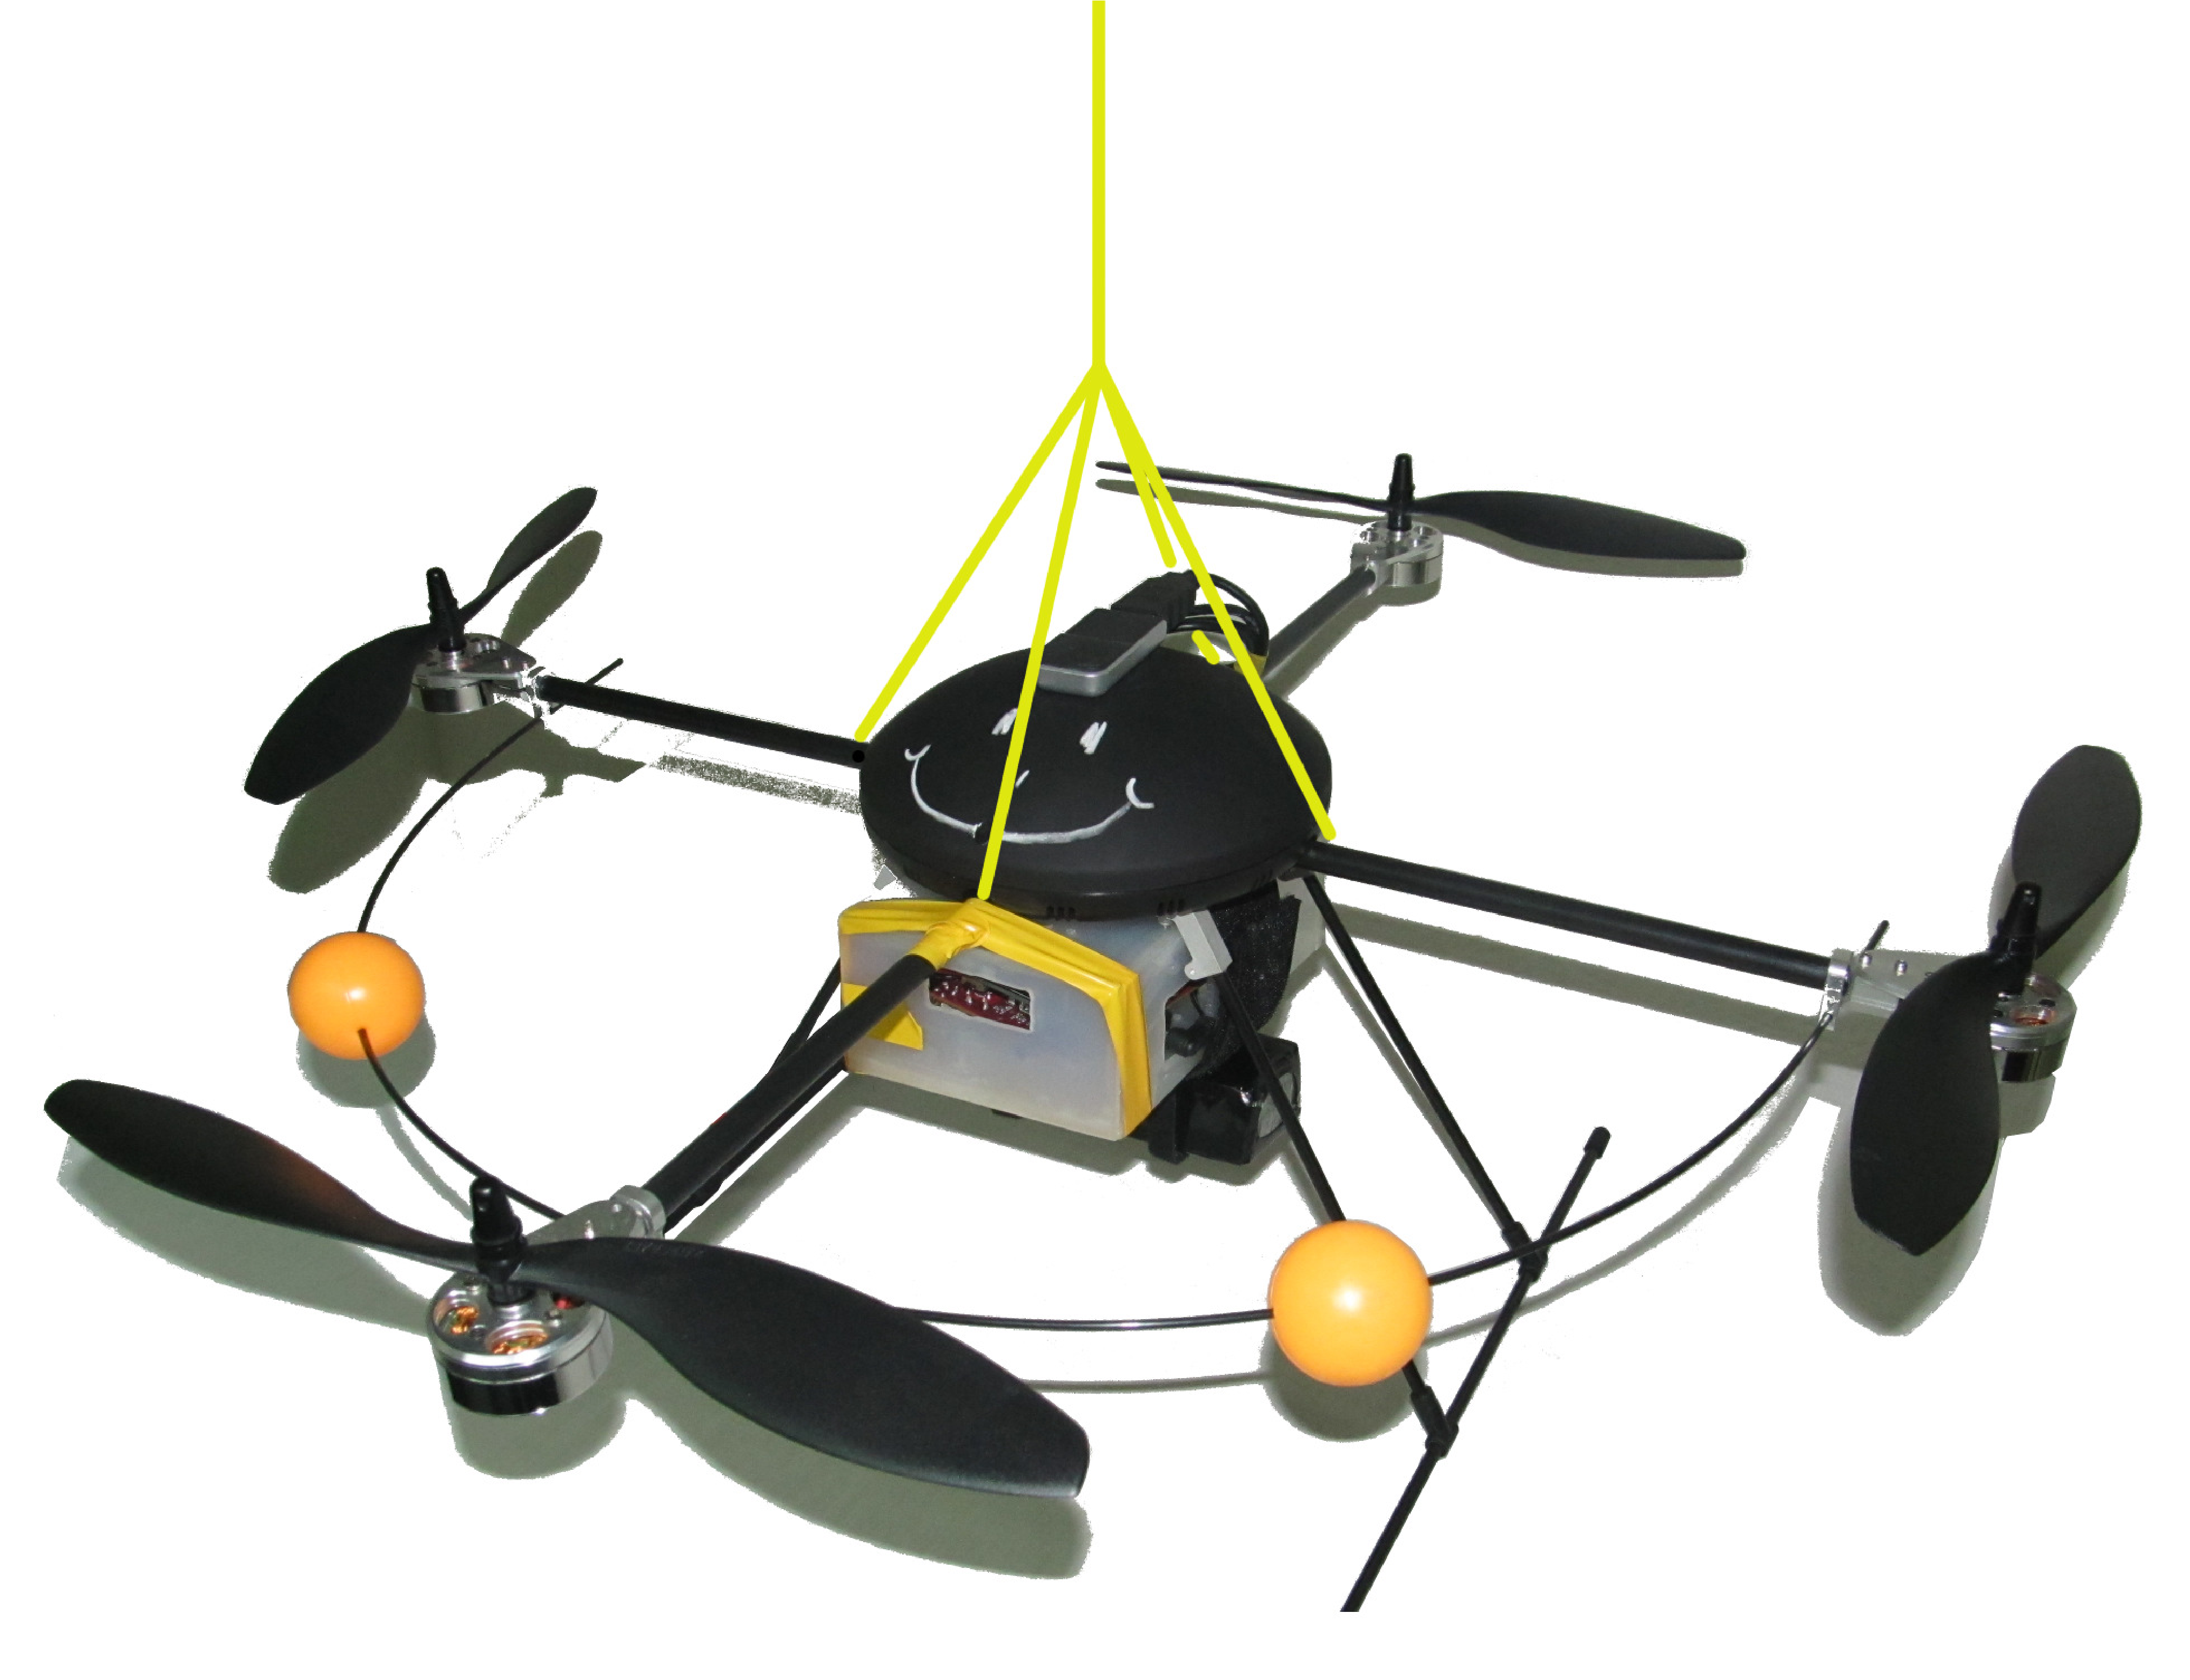
\includegraphics[width=0.4\textwidth]{./pics_test_control/dispositivo_theta.pdf}
	\caption{Dispositivo de prueba de $\theta$}
	\label{fig:thetadisp}
\end{wrapfigure}

El giro en $\theta$ es generado por un desequilibrio entre los pares ejercidos por las h\'elices. Si el par neto de todas las h\'elices resulta por ejemplo positivo, el cuadric\'optero realizar\'a un movimiento hacia los negativos, equilibrando el par, como se explica en el cap\'itulo \ref{chap:general}.\\

Para la estimaci\'on de $\theta$ se utiliza por un lado la integral de la velocidad angular en el eje ``z'' y por otro la proyecci\'on del vector del campo magn\'etico medido sobre el plano horizontal, medidas que son combinadas en el filtro de Kalman. El dato obtenido del magnet\'ometro no distingue entre giros de $360^o$, limitando el valor al rango [$-180^o$ : $180^o$]. Es necesario entonces realizar un reajuste de la medida deducida del campo magn\'etico para lograr la continuidad en el \'angulo estimado.\\

Análogamente a la parte anterior se realizan 2 pruebas, la primera dejando que el sistema alcance su posición de equilibrio en $\theta = \theta_{inicial}$, y la segunda apartándolo del equilibrio y dejándolo regresar a su punto de \emph{set point}.\\

El controlador, tal como sucede con los 2 ángulos anteriores ($\psi$ y $\phi$), consta de 2 términos proporcionales, uno para $\theta$ y otro para $w_{qz}$, además de un término integral en $\theta$. El subsistema queda descripto por la siguiente ecuación:
\begin{equation}
\left(\begin{array}{c}
\dot{\theta}\\
\dot{\omega}_{qz}\\
\dot{\theta_I}
\end{array}\right) = 
\left(\begin{array}{ccc}
0 & 1 & 0\\
0 & 0 & 0\\
1 & 0 & 0
\end{array}\right) 
\left(\begin{array}{c}
{\theta}\\
{\omega}_{qz}\\
{\theta_I}
\end{array}\right)
+ b\prime \left(\begin{array}{cccc}
0  & 0 &  0 & 0 \\
-1 & 1 & -1 & 1 \\
0  & 0 &  0 & 0
\end{array}\right) \left(\begin{array}{c}
\omega_1 \\
\omega_2 \\
\omega_3 \\
\omega_4
\end{array}\right)
\end{equation}

En este caso la matriz de realimentación utilizada es la siguiente:

\begin{equation}
\label{K_theta}
K = \left( \begin{array}{ccc}
-48.93 & -7.51 & -14.73\\
 48.93 &  7.51 &  14.73\\
-48.93 & -7.51 & -14.73\\
 48.93 &  7.51 &  14.73\\
\end{array}\right)
\end{equation}
\vspace{10pt}

Los resultados obtenidos se  muestran en las siguientes figuras. Se analiza en primer lugar el comportamiento del cuadricóptero dejándolo en equilibrio, luego se analiza la respuesta al escalón del subsistema en $\theta$ y por último se compara el comportamiento si se utiliza o no el término del integrador.

\begin{wrapfigure}{r}{0.6\textwidth}
	\vspace{-20pt}
	\centering
	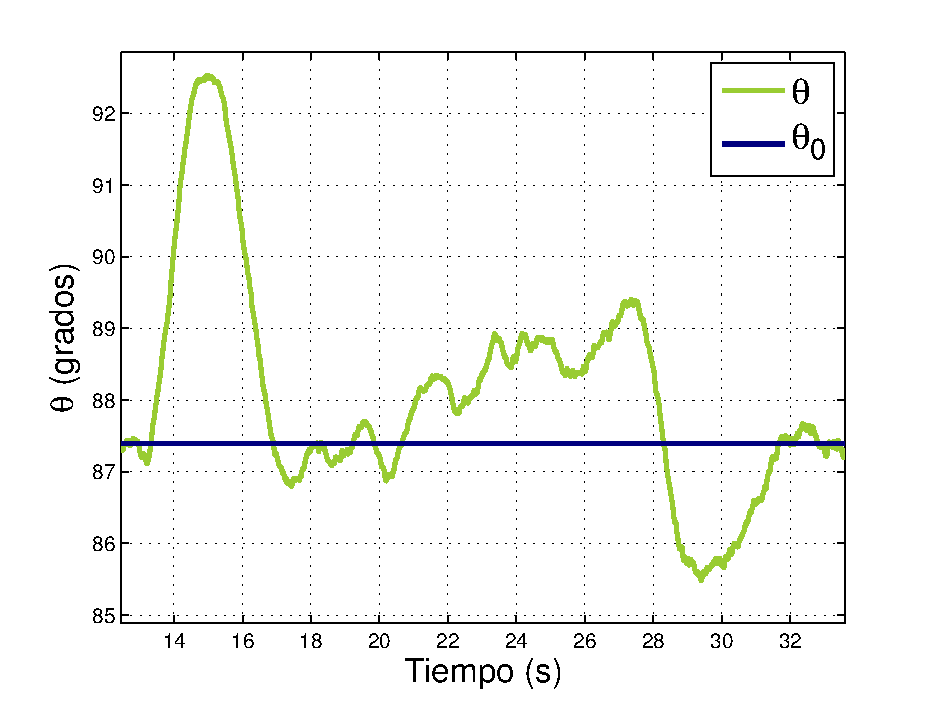
\includegraphics[width=0.52\textwidth]{./pics_test_control/theta.pdf}
	\caption{\'Angulo de Theta en lazo cerrado}
	\label{fig:theta}
\end{wrapfigure}

En la figura \ref{fig:theta} se observa la dinámica del ángulo $\theta$ obtenida en el dispositivo de prueba de la figura \ref{fig:thetadisp} utilizando un integrador en dicho ángulo. Nuevamente se puede observar un crecimiento al principio que es ocasionado por las diferencias de las respuestas de los motores. Rápidamente el integrador actúa integrando la diferencia con el \emph{set point} y corrigiendo el error cometido. Luego, en régimen, el ángulo en cuestión presenta un error típico de $\pm 2^\circ$, lo cual resulta aceptable.\\


\begin{wrapfigure}{l}{0.6\textwidth}
	\vspace{-10pt}
	\centering
	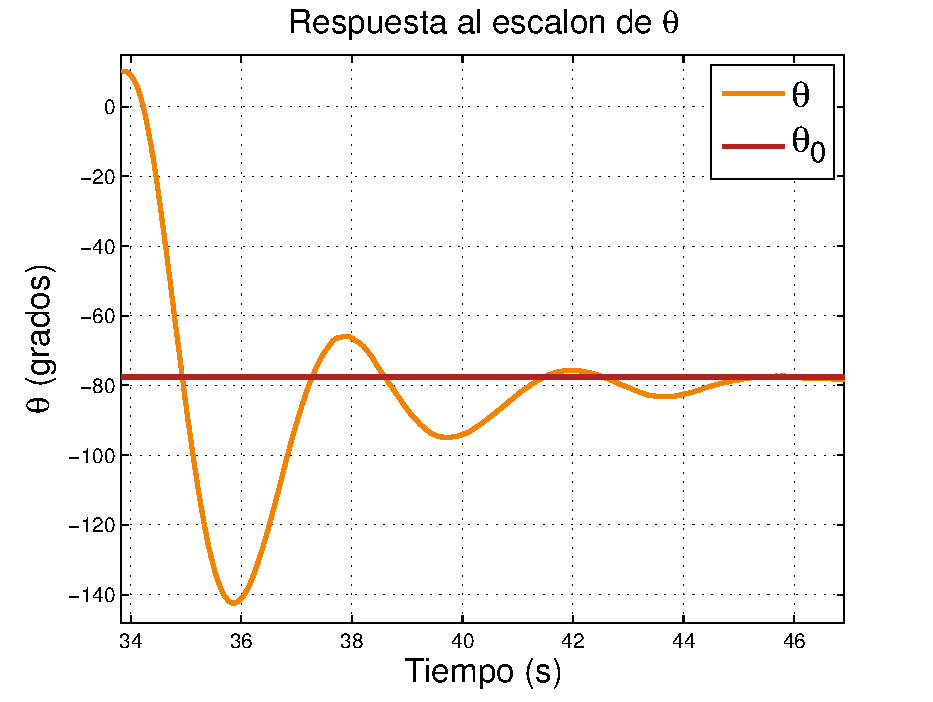
\includegraphics[width=0.52\textwidth]{./pics_test_control/theta_esc.pdf}
	\caption{Respuesta al escal\'on de Theta en\\ lazo cerrado}
	\label{fig:theta_esc}
\end{wrapfigure}

En la figura \ref{fig:theta_esc} se muestra la respuesta al escalón del ángulo en cuestión al apartarlo de su equilibrio aproximadamente $90^\circ$. Puede notarse claramente que el cuadricóptero vuelve a su equilibrio en forma satisfactoria en aproximadamente 6 segundos, tiempo que parece aceptable. Es importante destacar, de todas formas, que presenta un sobretiro considerable, alcanzando aproximadamente el 66\% del valor del escalón. Si bien es posible mejorar este aspecto, no resulta conveniente ya que en ese caso demora un tiempo sensiblemente mayor en volver al equilibrio. A su vez, el sobretiro en $\theta$ no parece ocasionar problemas de vuelo considerables para la mayoría de las aplicaciones.\\

\begin{wrapfigure}{r}{0.6\textwidth}
	\centering
	\vspace{-10pt}
	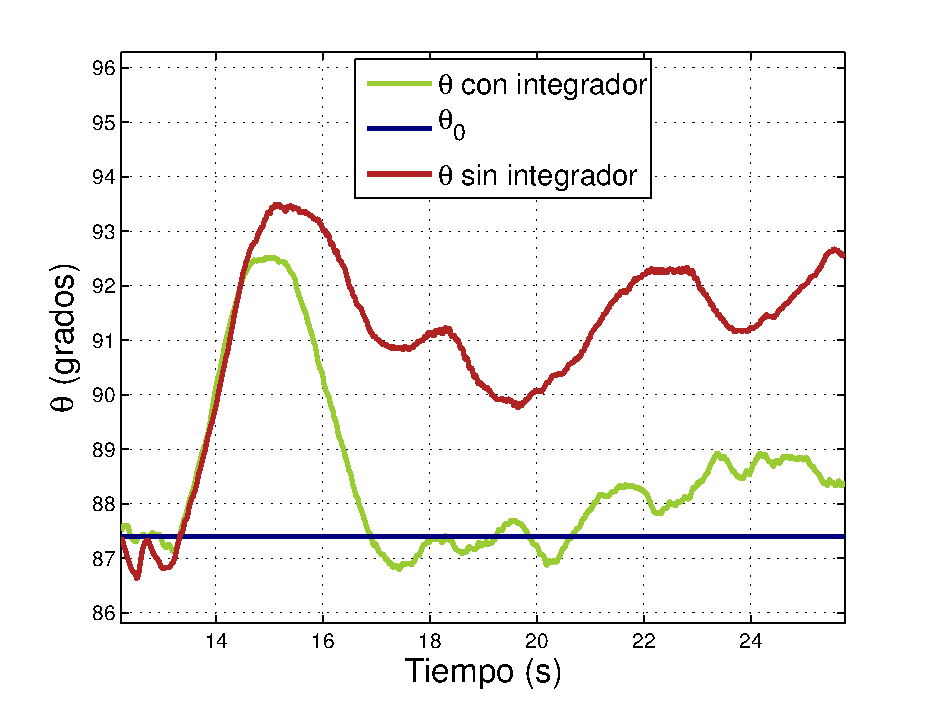
\includegraphics[width=0.52\textwidth]{./pics_test_control/theta_sin_con_int.pdf}
	\caption{\'Angulo de Theta en lazo cerrado}
	\vspace{-20pt}
	\label{fig:theta_sin_con_int}
\end{wrapfigure}

Por último en la figura \ref{fig:theta_sin_con_int} se evidencia la necesidad del término integral. Mientras que las diferencias entre los motores que ocasionan un aumento en el ángulo son corregidas rápidamente si se controla con el término integral, no ocurre lo mismo al utilizar un control solamente proporcional. Se puede observar que en este último caso el cuadricóptero llega a un equilibrio en $\theta$ distinto al \emph{set point}. A su vez el movimiento al inicio de dicho ángulo es mayor al utilizar el control solamente proporcional.\\

Al igual que en el análisis de \emph{Roll} y \emph{Pitch}, se concluye que la matriz de realimentación utilizada es adecuada para controlar de buena forma al ángulo \emph{Yaw}. \\

En la siguiente sección se presentarán los resultados del control completo del cuadricóptero en condiciones de vuelo, extendiendo la matriz a las variables de estado necesarias para lograr el control deseado.

\section{Control del sistema completo}
En las presentes pruebas el control realizado no incluye realimentaci\'on de la posici\'on $x$ e $y$ ni de las velocidades $v_{qx}$ y $v_{qy}$. Lo que se puede esperar con este controlador es que el sistema adquiera la orientaci\'on y la altura deseada, sin embargo es altamente probable que se produzca un desplazamiento horizontal. Al trabajar con el GPS se puede obtener una estimaci\'on m\'as adecuada de la posici\'on y de la velocidad horizontal y se la puede incluir en la realimentaci\'on, obteniendo as\'i un mejor controlador.\\

\begin{wrapfigure}{r}{0.6\textwidth}
	\centering
	\vspace{-20pt}
	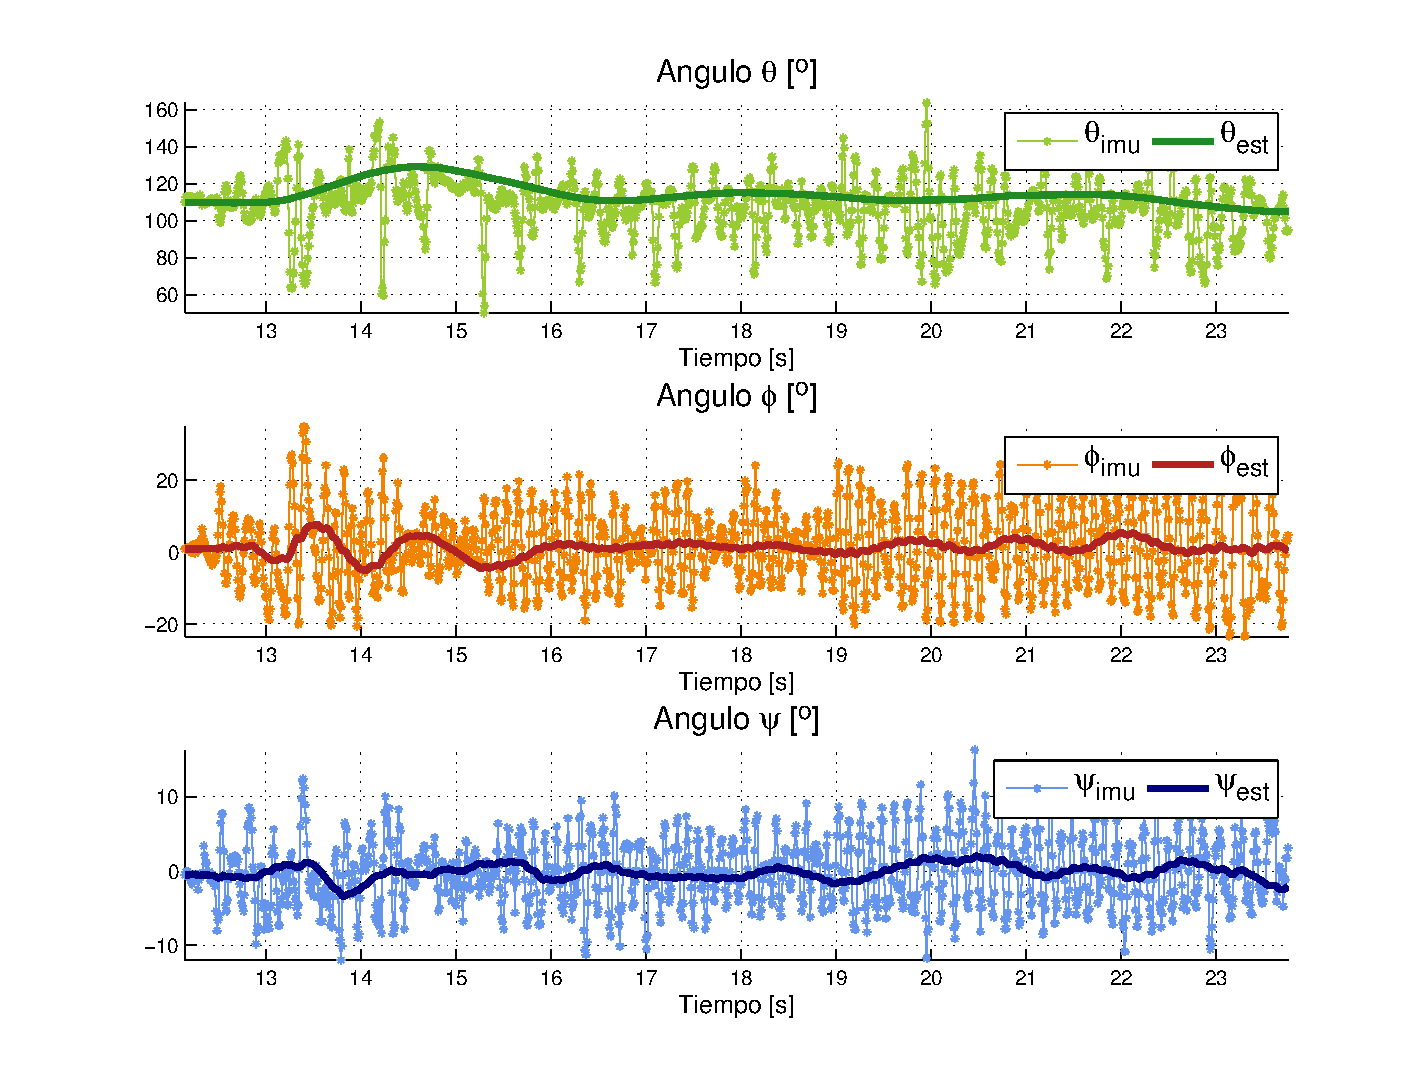
\includegraphics[width=0.52\textwidth]{./pics_test_control/euler.pdf}
	\caption{Ángulos de Euler}
	\label{fig:euler}
\end{wrapfigure}

En la figura \ref{fig:euler} se observa la medida y la estimaci\'on de los tres \'angulos de Euler a lo largo del tiempo de prueba en una situaci\'on de vuelo. Puede apreciarse claramente como el valor estimado de los \'angulos de Roll y Pitch mantienen valores cercanos a cero. El \'angulo de Pitch presenta en los primeros segundos de la prueba un comportamiento oscilatorio debido a la diferenca de empuje realizada por los motores de adelante y atras. Cinco segundos después de que empieza a funcionar el controlador (comienza a funcionar en el segundo once) se compensa este desperfecto logrando el equilibrio en torno al cero.

\begin{wrapfigure}{l}{0.55\textwidth}
	\centering
	\vspace{-15pt}
	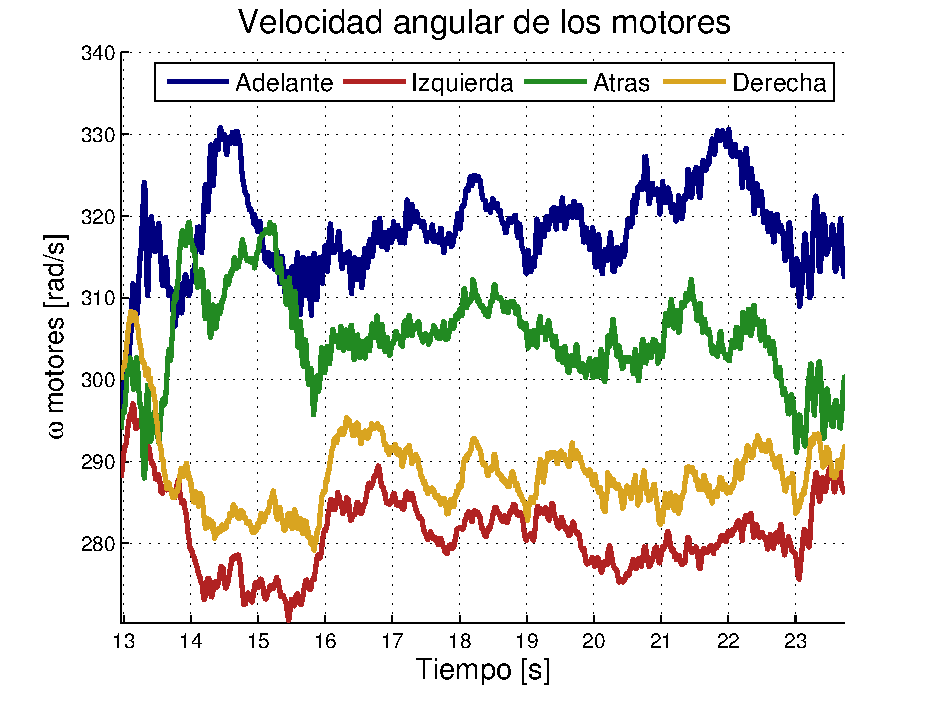
\includegraphics[width=0.52\textwidth]{./pics_test_control/w.pdf}
	\vspace{-15pt}
	\caption{$\omega$ de motores}
	\vspace{-20pt}
	\label{fig:w}
\end{wrapfigure}

En el caso del \'angulo de Yaw se observa que el mismo aumenta cerca de $20 ^\circ$ y luego se corrige, volviendo al valor de \emph{set point}. Se observ\'o que algunos motores no se encuentran perfectamente perpendiculares al plano horizontal del cuadric\'optero y la contribuci\'on de cada uno de los motores es tal que a la velocidad \'angular de \emph{set point} se produce un giro seg\'un $k_q$.\\ 

Este desperfecto se corrige con el integrador en el \'angulo de Yaw. En la figura \ref{fig:w} se observa claramente el aumento de las velocidades angulares de los motores de adelante y atras y la disminuci\'on en los motores laterales.\\ 

\begin{wrapfigure}{l}{0.6\textwidth}
	\centering
	\vspace{-10pt}
	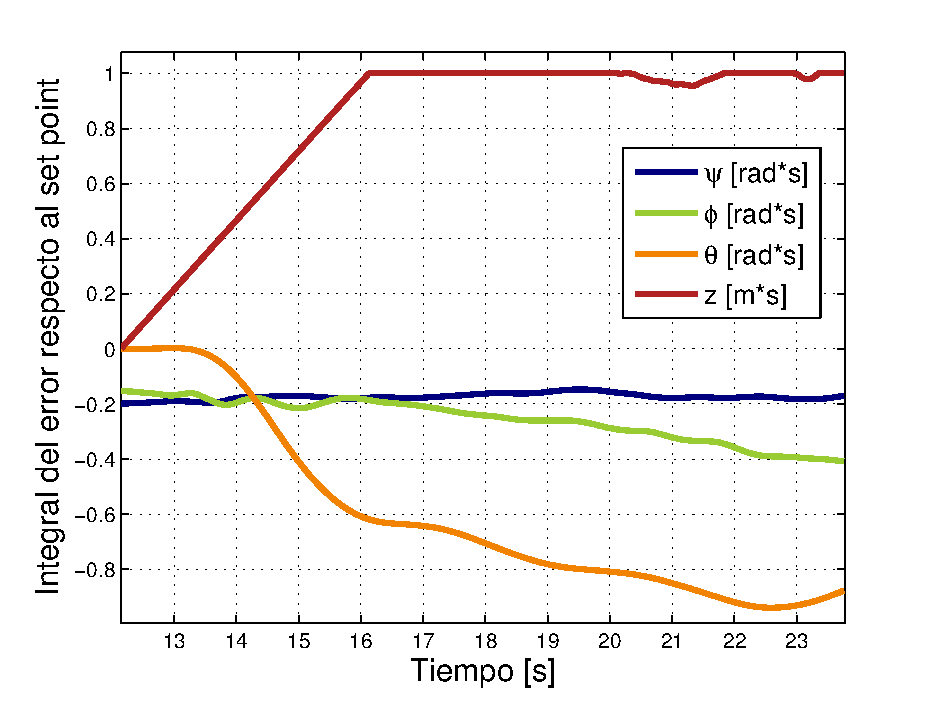
\includegraphics[width=0.52\textwidth]{./pics_test_control/int.pdf}
	\caption{Integrales}
	\label{fig:int}
\end{wrapfigure}

En la figura \ref{fig:int} se observa como el valor de la integral del error cometido en el \'angulo de Yaw aumenta en m\'odulo hasta que en alrededor del segundo 19 de la prueba comienza a estabilizarse. Este valor de la integral del error es el responsable del comportamiento descripto anteriormente.\\

El integrador permite tambi\'en explicar la compensaci\'on de la diferencia de empuje entre los motores de adelante y atr\'as. Recordamos el comportamiento oscilatorio del \'angulo de Pitch en los segundos iniciales de la prueba de vuelo, donde presentaba un offset positivo. La explicaci\'on de este fen\'omeno es que el empuje del motor de atr\'as es mayor que el de adelante. En la figura \ref{fig:int}, se observa como la integral del error en el \'angulo de Pitch ($\varphi$) disminuye, confirmando la observaci\'on anterior. A su vez en la figura \ref{fig:w} se observa que existe una diferencia en las velocidades angulares seteadas en los motores en cuesti\'on. Se fija un valor mayor para el motor de adelante que para el de atr\'as a fin de compensar este efecto. Sucede algo similar aunque en menor medida para el \'angulo de Roll ($\psi$) y los motores laterales.\\ 

\begin{wrapfigure}{l}{0.6\textwidth}
	\centering
	\vspace{-10pt}
	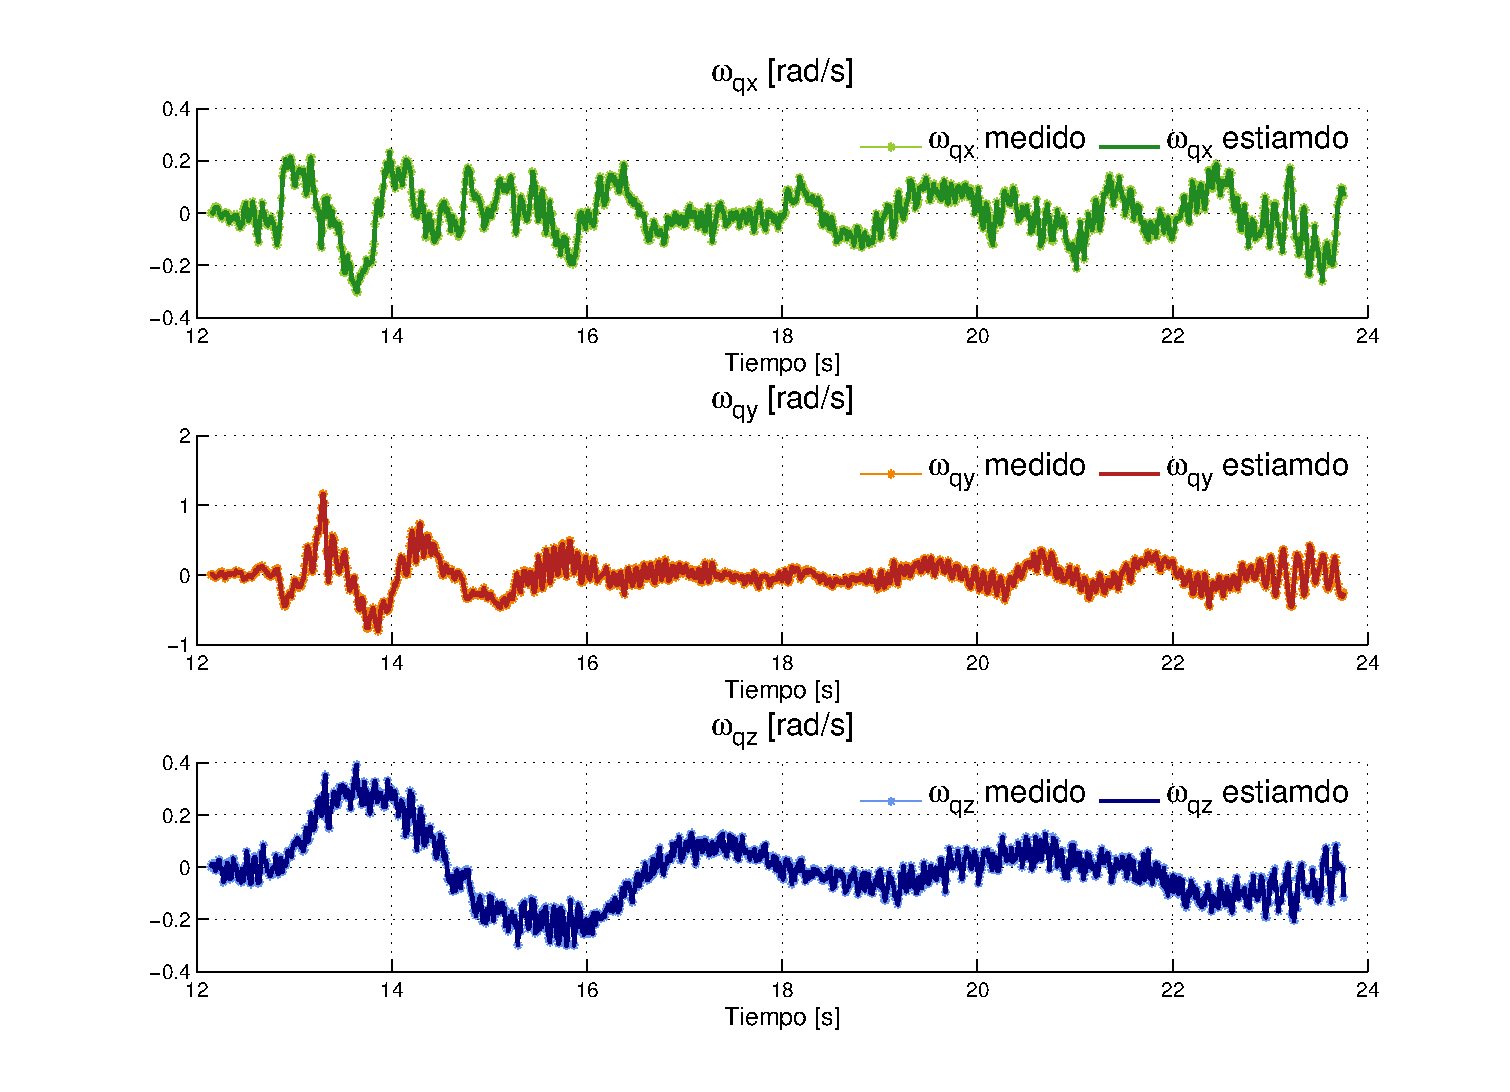
\includegraphics[width=0.55\textwidth]{./pics_test_control/wq.pdf}
	\caption{Velocidades angulares del\\cuadricóptero}
	\label{fig:wq}
\end{wrapfigure}

En lo que respecta a las velocidades angulares del sistema puede observarse que en los tres casos las mismas se encuentran en valores cercanos al cero. En los primeros segundos se obtienen algunas variaciones fundamentalmente en $\omega_{qy}$ y $\omega_{qz}$. Este resultado se condice con lo observado anteriormente. Incluso se observa que el andamiento de las curvas de velocidades angulares se corresponde con la derivada de los \'angulos de Euler, por lo que estos resultados se adecuan perfectamente a lo esperado.\\

A partir de los resultados analizados hasta el momento se puede asegurar que el control realizado sobre el subsistema de los \'angulos de Euler y las velocidades angulares del cuadric\'optero en situaci\'on de \emph{hovering} es satisfactorio. Volvemos a hacer \'enfasis en la importancia de este subsistema ya que es aquel que garantiza la estabilidad del cuadric\'optero. Errores en la posici\'on pueden no ser tan importantes ya que si no se logra una posici\'on determinada pero se alcanza una cercana, el resultado global puede ser satisfactorio en una amplia gama de aplicaciones. Este no es el caso del subsistema de los \'angulos (fundamentalmente el de los \'angulos de Roll y de Pitch). Errores en estos \'angulos producen la deriva del sistema o incluso que el sistema no pueda mantenerse en vuelo. \\
\begin{wrapfigure}{l}{0.6\textwidth}
	\centering
	\vspace{-10pt}
	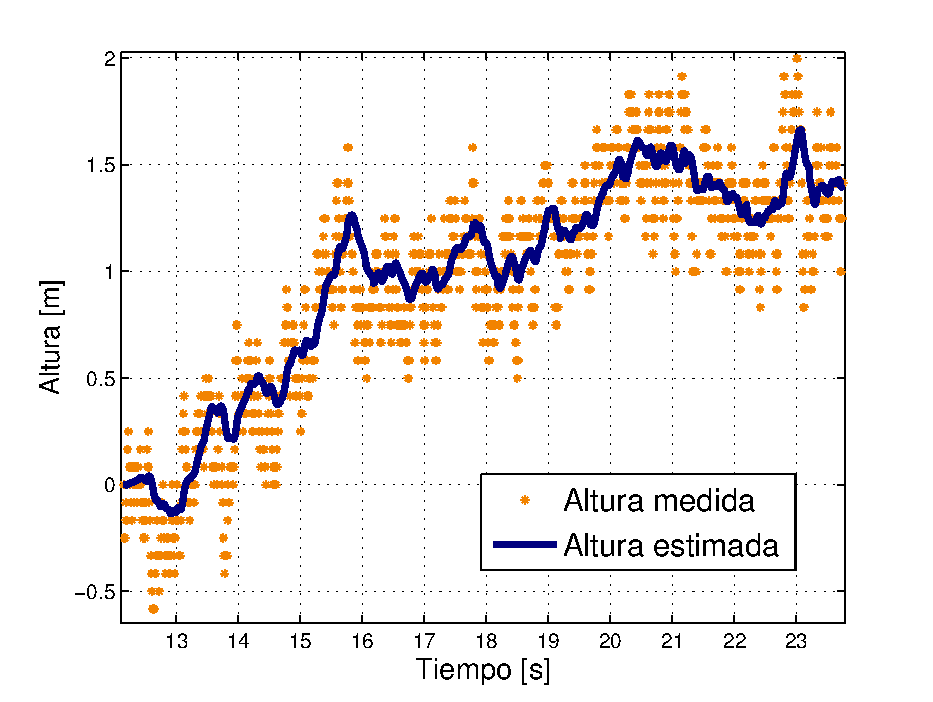
\includegraphics[width=0.52\textwidth]{./pics_test_control/z.pdf}
	\caption{Altura}
	\label{fig:z}
\end{wrapfigure}

Por último se centrará la atención en analizar la altura. En la presente prueba se establece como valor objetivo de la altura $1.5m$. En la figura \ref{fig:z} se observa que el valor objetivo es alcanzado en aproximadamente cinco segundos. Nuevamente, cabe destacar la importancia del integrador en la altura. En la figura \ref{fig:int} puede observarse la integral del error en la altura alcanza el valor m\'aximo permitido. En esta situaci\'on se est\'a seteando una velocidad angular mayor a la que se hubiera seteado sin agregar el integrador. Esto implica que sin el integrador no se hubiera podido alcanzar la altura objetivo, logrando un equilibrio a una altura inferior. Como se explic\'o en el cap\'itulo \ref{chap:control}, sin el integrador, variaciones en la masa o errores en la caracterizaci\'on del empuje de los motores implican puntos de equilibrio distintos. \\

En esta secci\'on se pudo verificar el correcto funcionamiento del control diseñado. En esta prueba, como fue aclarado previamente, no se realimenta la informaci\'on de posiciones y velocidades horizontales. Los resultados obtenidos son satisfactorios permitiendo al sistema mantener el equilibrio en per\'iodos donde la señal de GPS no se encuentra disponible o se encuentran disponibles muy pocos sat\'elites conduciendo a medidas con errores superiores a lo deseado. Este controlador permite ignorar datos del GPS si estos est\'an muy contaminados por ru\'ido.\\

El control con señal de GPS no pudo ser verificado, pero es de esperar su correcto funcionamiento debido a que las simulaciones arrojan buenos resultados.








\end{document}